% -*- TeX-command-extra-options: "-shell-escape"; -*-
\documentclass[convert={density=1200,size=1080x800,outext=.png}, tikz]{standalone}
\usetikzlibrary{matrix}
\usetikzlibrary{angles, quotes}
\usetikzlibrary{calc, positioning}
% \usetikzlibrary{arrows.meta}
\begin{document}
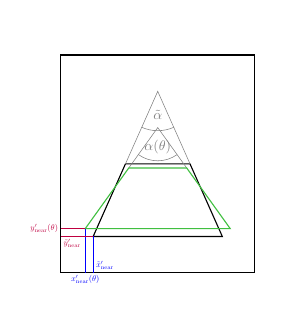
\begin{tikzpicture}

  \matrix (grid) [matrix of nodes, transparent=1]
  {
    8 & 8 & 8 & 8 & 1 & 6 & 6 \\
    8 & 8 & 8 & 8 & 1 & 6 & 6 \\
    8 & 8 & 8 & 8 & 1 & 6 & 6 \\
    3 & 3 & 3 & 3 & 5 & 7 & 7 \\
    4 & 4 & 4 & 4 & 9 & 2 & 2 \\
    4 & 4 & 4 & 4 & 9 & 2 & 2 \\
    4 & 4 & 4 & 4 & 9 & 2 & 2 \\
  };

  % runway outline
  \draw (grid-6-2.center)
  to (grid-4-3.center)
  to (grid-4-5.center)
  to (grid-6-6.center)
  to cycle;


  % runway extensions
  \draw[gray, very thin]
  (grid-4-3.center) coordinate (A) to
  (grid-2-4.center) coordinate (B) to
  (grid-4-5.center) coordinate (C)
  pic ["$\tilde{\alpha}$"scale=0.5, draw, solid] {angle};
  % \draw[gray, dashed, very thin, shorten <=1pt] (grid-3-4.center) to (grid-1-3.center);

  \coordinate (pred-vanish) at ($(grid-3-4)!0.0!(grid-4-4)$);
  % \draw[red] (pred-vanish) circle[radius=1pt];
  \coordinate (pred-near-left)  at ($(grid-6-2)+(-0.1, 0.1)$);
  % \draw[red] (pred-near-left) circle[radius=1pt];
  \coordinate (pred-near-right) at ($(grid-6-6)+(+0.1, 0.1)$);
  % \draw[red] (pred-near-right) circle[radius=1pt];

  \coordinate (pred-far-left)  at  ($(pred-near-left)!0.6!(pred-vanish)$);
  \coordinate (pred-far-right) at ($(pred-near-right)!0.6!(pred-vanish)$);
  \draw[gray, very thin]
  (pred-far-left) coordinate (A) to
  (pred-vanish) coordinate (B) to
  (pred-far-right) coordinate (C)
  pic ["$\alpha(\theta)$"scale=0.5, draw, solid, angle radius=12] {angle};

  \draw[gray!50!green]
  (pred-near-left)  to
  (pred-far-left)  to
  (pred-far-right) to
  (pred-near-right) to
  cycle;

  \draw (grid-1-1.center) to (grid-7-1.center) to (grid-7-7.center) to (grid-1-7.center) to cycle;

  \draw[very thin, blue] (pred-near-left) to (pred-near-left |- grid-7-1.center) node[anchor=north,  scale=0.3] {$x'_{\rm near}(\theta)$};
  \draw[very thin, blue] (grid-6-2.center) to (grid-6-2.center |- grid-7-1.center) node[anchor=south west,  scale=0.3] {$\tilde{x}'_{\rm near}$};

  \draw[very thin, purple] (pred-near-left) to (pred-near-left -| grid-7-1.center) node[anchor=east,  scale=0.3] {$y'_{\rm near}(\theta)$};
  \draw[very thin, purple] (grid-6-2.center) to (grid-6-2.center -| grid-7-1.center) node[anchor=north west,  scale=0.3] {$\tilde{y}'_{\rm near}$};


\end{tikzpicture}
\end{document}
